\documentclass[11pt,letter]{article}
%--------------図を挿入するための設定等々-----------
\usepackage{amsmath,amssymb}
%\usepackage[hidelinks]{hyperref}
\usepackage{hyperref}
\usepackage{amsthm}
\usepackage{hvfloat}
\usepackage{mathrsfs}
\usepackage{bm}
\usepackage{ascmac} 
\usepackage{amsmath}
\usepackage{natbib} %経済学用bibtexスタイル
\usepackage{fancybox}
\usepackage{float}
\usepackage{booktabs} 
\usepackage{bm,xstring}
\usepackage{tabularx}
\usepackage{graphicx}
%\usepackage{mediabb}
\usepackage{lipsum}
\usepackage {pdfpages}
\usepackage{booktabs}
\usepackage{array}
\usepackage{paralist}
\usepackage{verbatim}
\usepackage{subfig} 
\usepackage{ascmac}
\usepackage{amsthm}
\usepackage{multirow}
\usepackage{amsmath}
\usepackage{natbib}
\usepackage{longtable}
\usepackage{hhline}
\usepackage{tabularx}
\usepackage{booktabs}
%\usepackage[T1]{fontenc}
\usepackage{textcomp}
\usepackage{here}
\usepackage{setspace}
\usepackage{color}
\usepackage{url}
\usepackage{xcolor}
%\usepackage{filecontents}
\usepackage{setspace}
\usepackage{fancyhdr}
\usepackage{titling}
\usepackage{titlesec}
\usepackage{sectsty}
\usepackage{listings}
\usepackage[many]{tcolorbox}
\usepackage[framemethod=TikZ]{mdframed}
\usepackage[dvipdfmx]{}
%\usepackage[dvipdfmx]{color}
\usepackage[flushleft]{threeparttable} % Table note
%\usepackage[dvipdfmx]{color}
\usepackage[title]{appendix}
\usepackage{bbm}
\usepackage{pdflscape}
\newcommand{\vect}[1]{\boldsymbol{\mathbf{#1}}}

\usepackage{appendix}

%%%%%%%%%%%%%%%%%%%%%%%%%%%%%%
%Theorem
\newcounter{theo}[section] \setcounter{theo}{0}
\renewcommand{\thetheo}{\arabic{theo}}
\newenvironment{theo}[2][]{%
\refstepcounter{theo}%
\ifstrempty{#1}%
{\mdfsetup{%
frametitle={%
\tikz[baseline=(current bounding box.east),outer sep=0pt]
\node[anchor=east,rectangle,fill=gray!20]
{\strut Theorem~\thetheo};}}
}%
{\mdfsetup{%
frametitle={%
\tikz[baseline=(current bounding box.east),outer sep=0pt]
\node[anchor=east,rectangle,fill=gray!20]
{\strut Theorem~\thetheo:~#1};}}%
}%
\mdfsetup{innertopmargin=10pt,linecolor=gray!20,%
linewidth=2pt,topline=true,%
frametitleaboveskip=\dimexpr-\ht\strutbox\relax
}
\begin{mdframed}[]\relax%
\label{#2}}{\end{mdframed}}
%%%%%%%%%%%%%%%%%%%%%%%%%%%%%%
%Lemma
\newcounter{lem}[section] \setcounter{lem}{0}
\renewcommand{\thelem}{\arabic{section}.\arabic{lem}}
\newenvironment{lem}[2][]{%
\refstepcounter{lem}%
\ifstrempty{#1}%
{\mdfsetup{%
frametitle={%
\tikz[baseline=(current bounding box.east),outer sep=0pt]
\node[anchor=east,rectangle,fill=gray!50]
{\strut Lemma~\thelem};}}
}%
{\mdfsetup{%
frametitle={%
\tikz[baseline=(current bounding box.east),outer sep=0pt]
\node[anchor=east,rectangle,fill=gray!50]
{\strut Lemma~\thelem:~#1};}}%
}%
\mdfsetup{innertopmargin=10pt,linecolor=gray!50,%
linewidth=2pt,topline=true,%
frametitleaboveskip=\dimexpr-\ht\strutbox\relax
}
\begin{mdframed}[]\relax%
\label{#2}}{\end{mdframed}}
%%%%%%%%%%%%%%%%%%%%%%%%%%%%%%
%Assumption
\newcounter{asm}[section] \setcounter{asm}{0}
\renewcommand{\theasm}{\arabic{section}.\arabic{asm}}
\newenvironment{asm}[2][]{%
\refstepcounter{asm}%
\ifstrempty{#1}%
{\mdfsetup{%
frametitle={%
\tikz[baseline=(current bounding box.east),outer sep=0pt]
\node[anchor=east,rectangle,fill=gray!50]
{\strut Assumption~\theasm};}}
}%
{\mdfsetup{%
frametitle={%
\tikz[baseline=(current bounding box.east),outer sep=0pt]
\node[anchor=east,rectangle,fill=gray!50]
{\strut Assumption~\thelem:~#1};}}%
}%
\mdfsetup{innertopmargin=10pt,linecolor=gray!50,%
linewidth=2pt,topline=true,%
frametitleaboveskip=\dimexpr-\ht\strutbox\relax
}
\begin{mdframed}[]\relax%
\label{#2}}{\end{mdframed}}
%%%%%%%%%%%%%%%%%%%%%%%%%%%%%%
%Definition
\newcounter{defn}[section] \setcounter{defn}{0}
\renewcommand{\thedefn}{\arabic{section}.\arabic{defn}}
%\renewcommand{\thedefn}{\arabic{defn}}
\newenvironment{defn}[2][]{%
\refstepcounter{defn}%
\ifstrempty{#1}%
{\mdfsetup{%
frametitle={%
\tikz[baseline=(current bounding box.east),outer sep=0pt]
\node[anchor=east,rectangle,fill=gray!50]
{\strut Definition~\thedefn};}}
}%
{\mdfsetup{%
frametitle={%
\tikz[baseline=(current bounding box.east),outer sep=0pt]
\node[anchor=east,rectangle,fill=gray!50]
{\strut Definition~\thedefn:~#1};}}%
}%
\mdfsetup{innertopmargin=10pt,linecolor=gray!50,%
linewidth=2pt,topline=true,%
frametitleaboveskip=\dimexpr-\ht\strutbox\relax
}
\begin{mdframed}[]\relax%
\label{#2}}{\end{mdframed}}

%%%%%%%%%%%%%%%%%%%%%%%%%%%%%%
%Proof
\newcounter{prf}[section]\setcounter{prf}{0}
\renewcommand{\theprf}{\arabic{section}.\arabic{prf}}
\newenvironment{prf}[2][]{%
\refstepcounter{prf}%
\ifstrempty{#1}%
{\mdfsetup{%
frametitle={%
\tikz[baseline=(current bounding box.east),outer sep=0pt]
\node[anchor=east,rectangle,fill=gray!50]
{\strut Proof~\theprf};}}
}%
{\mdfsetup{%
frametitle={%
\tikz[baseline=(current bounding box.east),outer sep=0pt]
\node[anchor=east,rectangle,fill=gray!50]
{\strut Proof~\theprf:~#1};}}%
}%
\mdfsetup{innertopmargin=10pt,linecolor=gray!50,%
linewidth=2pt,topline=true,%
frametitleaboveskip=\dimexpr-\ht\strutbox\relax
}
\begin{mdframed}[]\relax%
\label{#2}}{\qed\end{mdframed}}
%%%%%%%%%%%%%%%%%%%%%%%%%%%%%%
%%%%%%%%%%%%%%%%%%%%%%%%%%%%%%
%Note
\newcounter{notes}[section] \setcounter{notes}{0}
\renewcommand{\thenotes}{\arabic{notes}}
\newenvironment{notes}[2][]{%
\refstepcounter{notes}%
\ifstrempty{#1}%
{\mdfsetup{%
frametitle={%
\tikz[baseline=(current bounding box.east),outer sep=0pt]
\node[anchor=east,rectangle,fill=gray!50]
{\strut Note~\thenotes};}}
}%
{\mdfsetup{%
frametitle={%
\tikz[baseline=(current bounding box.east),outer sep=0pt]
\node[anchor=east,rectangle,fill=gray!50]
{\strut Note~\thenotes:~#1};}}%
}%
\mdfsetup{innertopmargin=10pt,linecolor=gray!50,%
linewidth=2pt,topline=true,%
frametitleaboveskip=\dimexpr-\ht\strutbox\relax
}
\begin{mdframed}[]\relax%
\label{#2}}{\end{mdframed}}

\newtcolorbox{myboxi}[1][]{
  breakable,
  title=#1,
  colback=white,
  colbacktitle=white,
  coltitle=black,
  fonttitle=\bfseries,
  bottomrule=0pt,
  toprule=0pt,
  leftrule=3pt,
  rightrule=3pt,
  titlerule=0pt,
  arc=0pt,
  outer arc=0pt,
  colframe=black,
}

%フォント
\usepackage{tgpagella}

\definecolor{mygreen}{RGB}{28,172,0} % color values Red, Green, Blue
\definecolor{mylilas}{RGB}{170,55,241}
\lstset{language=Matlab,%
    %basicstyle=\color{red},
    breaklines=true,%
    morekeywords={matlab2tikz},
    keywordstyle=\color{blue},%
    morekeywords=[2]{1}, keywordstyle=[2]{\color{black}},
    identifierstyle=\color{black},%
    stringstyle=\color{mylilas},
    commentstyle=\color{mygreen},%
    showstringspaces=false,%without this there will be a symbol in the places where there is a space
    numbers=left,%
    numberstyle={\tiny \color{black}},% size of the numbers
    numbersep=9pt, % this defines how far the numbers are from the text
    emph=[1]{for,end,break},emphstyle=[1]\color{red}, %some words to emphasise
    %emph=[2]{word1,word2}, emphstyle=[2]{style},    
}

%\usepackage[none]{hyphenat}
\usepackage{geometry}
\geometry{left=1in,right=1in, top=1in,bottom=1in}
%\setlength\parindent{0pt}
%\renewcommand{\thesubsection}{(\alph{subsection})}
\usepackage{fancyhdr}
 

%\usepackage[shortlabels]{enumitem}
%                    \setlist[enumerate, 1]{1\textsuperscript{o}}


%--------------ショートカット-----------
%Expectation
\newcommand{\Exp}[1]{\mathbb{E}\left[{#1}\right]}
\newcommand{\Var}[1]{\text{Var}\left[{#1}\right]}
\newcommand{\AsymVar}[1]{\text{AsymVar}\left[{#1}\right]}
\newcommand{\cov}[1]{\text{cov}\left[{#1}\right]}
\newcommand{\plim}[1]{\text{plim}\{{#1}\}}
\newcommand{\Ind}[1]{\mathbbm{1}\{{#1}\}}
\newcommand{\Prob}[1]{\text{Pr}\left({#1}\right)}
%hat
\newcommand{\h}[1]{\hat{#1}}

%upper and lower ber
\newcommand{\ob}[1]{\overline{#1}}
\newcommand{\ub}[1]{\underline{#1}}
\newcommand{\taubar}{\overline{\tau}}

%epsilon
\newcommand{\epsi}{\varepsilon}
\def\checkmark{\tikz\fill[scale=0.4](0,.35) -- (.25,0) -- (1,.7) -- (.25,.15) -- cycle;} 

\newcommand{\nonum}{\nonumber}

%ln()
\newcommand{\lnp}[1]{\ln\left({#1}\right)}

% parenthesis
\newcommand{\prn}[1]{\left({#1}\right)}
\newcommand{\mprn}[1]{\{{#1}\}}
\newcommand{\lmprn}[1]{\big\{{#1}\big\}}
\newcommand{\Lmprn}[1]{\Big\{{#1}\Big\}}
\newcommand{\llmprn}[1]{\biggl\{{#1}\biggr\}}
\newcommand{\LLmprn}[1]{\Biggl\{{#1}\Biggr\}}
\newcommand{\lprn}[1]{\left[{#1}\right]}

% cfrac
\newcommand{\cf}[2]{\cfrac{#1}{#2}}

% convergence in probability
\newcommand{\conp}{\xrightarrow{p}}
\newcommand{\cond}{\xrightarrow{d}}

% Norm
\newcommand{\norm}[1]{\left\lVert{#1}\right\rVert}
\newcommand{\abs}[1]{\left\lvert{#1}\right\rvert}

\newcommand{\rootn}{\sqrt{n}}

\newcommand{\note}[1]{\ \ \ \ \text{#1}}

\newcommand{\ave}[1]{\frac{1}{#1}\sum_{i=1}^{#1}}

\newcommand{\half}{\cfrac{1}{2}}
\newcommand{\pihat}{\hat{\pi}}

\newcommand{\mbf}[1]{\mathbf{#1}}

\DeclareMathOperator*{\argmax}{argmax} 
\DeclareMathOperator*{\argmin}{argmin} 

\newcommand{\pmat}[1]{\begin{pmatrix} #1 \end{pmatrix}}%行列簡略化
\newcommand{\bmat}[1]{\begin{bmatrix} #1 \end{bmatrix}}%行列簡略化

\pagestyle{fancy}
\fancyhf{}
\chead{}
\rhead{Empirical Methods Project (K. Suzuki)}
\lhead{ECON512: Empirical Method (Prof. Grieco)}
\cfoot{\thepage}
%\allowdisplaybreaks
%\setstretch{1.5}

\newtheorem{definition}{Definition}

%--------------タイトル開始-----------
\title{Productivity Implication of Importing Intermediate and Fixed Cost of Import: Evidence from Chinese Firm-Level Data}
\author{Kensuke Suzuki\thanks{ % Thanks
			This study is undertaken as an empirical methods project in ECON512 Empirical Methods (Professor Paul Grieco) and a mini-research project in ECON570 Development Economics (Professor Kala Krishna). The China Industrial Firm Statistics Dataset and China Custom Export-Import Dataset are provided by Professor Hong Ma at Tsinghua University.}
						}
\date{\today}
\begin{document}

\bibliographystyle{aer} 

%--------------文章開始-----------


%%%%%%%%%%%%%%%%%%%%%%%%%%%%

\maketitle

%\begin{center}China Expo
%\Large{Note: estimating fixed cost of import}\\
%\large{Ken Suzuki}\\
%\large{\today}
%\end{center}

%%%%%%%%%%%%%%%%%%%%
\section{Motivation}

Firm's decision on importing intermediate inputs and its productivity implication have been widely discussed in the literature of development economics and international trade. Provided the empirical regularity from firm-level data showing that importers are likely to be larger and more productive than non-importers \citep{Bernard2012}, these studies build upon a model with firm heterogeneity in productivity.  

In the standard \citeauthor{Melitz2003} type of firm heterogeneity model, selection of firms into importing can be explained by the existence of fixed and sunk costs of import, i.e., firm needs to incur the sunk and fixed cost to initiate and keep foreign sourcing. Only firms that are sufficiently productive find it profitable to import intermediate goods. 

However, this productivity sorting is not perfect in the data. Looking at Chinese firm-level data, I found that productivity distributions of importers and non-importers are substantially overlapping.\footnote{In Appendix \ref{empresult}, I present the tentative result for the production function estimation \textit{\`a la} \citet{Levinsohn2003}. Figure 1 and 2 show the productivity distributions (histograms) of importers and non-importers.} In other words, there are large mass of high productive, but not importing firms. This imperfect sorting can be attributed to the heterogeneity of fixed and sunk cost of import.\footnote{The other rationale would be the possibility of vertical integration by the high productive firms, which is beyond the scope of this study.} For example, conditional on firm's productivity, a firm which draws higher fixed cost would not be able to import intermediate goods from abroad.

Given this emphasis, in this study, I introduce the stochastic formulation of fixed and sunk cost of import into the structural model of firm's importing behavior. I estimate the model using Chinese firm level data. This will allow us to assess how importing intermediate inputs affects the evolution of firm's productivity and how heterogeneous the fixed and sunk costs of import are.


%%%%%%%%%%%%%%%%%%%%%%%%%%%%%%%%%%%%
\section{Theoretical Framework}

The basic framework of the model is based on \citet{Kasahara2008}. The full description of the model is presented in Appendix \ref{model}. I assume that intermediate inputs are aggregated by the standard CES aggregator. Since importers would be able to access wider variety of inputs than non-importers, this captures the static benefit of importing intermediate inputs. Provided that the dataset does not contain product-level intermediate inputs, I assume an equilibrium where all the intermediate inputs are used symmetrically. This allows us to distinguish importers from non-importers by the relative measure of total intermediate inputs to domestically produced intermediate inputs. Importing also has dynamic implication, i.e., the evolution of firm's productivity depends on the previous period productivity and import decision. This captures the \textit{learning by importing effect}. The major departure from \citeauthor{Kasahara2008}'s model is that I introduce stochastic specification of fixed and sunk cost of import, i.e., a firm draws a relevant cost (i.e., startup sunk cost or fixed cost) of import depending on the previous period import decision. This formulation is inspired by \citet{Bai2017}. Upon observing the cost, a firm solves dynamic optimization problem and decide whether to import.

%%%%%%%%%%%%%%%%%%%%%%%%%%%%%%%%%%%%
\section{Data}

I use two Chinese data sets. The first one consist of firm-level data from the Annual Survey of Industrial Production (ASIP) from 1998 to 2007 conducted by the Chinese government's National Bureau of Statistics. The data contains information on the firm's industry of production, ownership type, employment, capital stocks, and revenues. The second data set is Chinese Customs transaction-level data. It records the universe of transaction by Chinese firms that participated in international trade over the 2000--2006 period. Detailed description is available in Appendix \ref{data}.

In the empirical analysis, I focus on the manufacturing of electrical machinery (\#31 of 2-digit ISIC Rev.3). I choose this industry after taking into account the number of observations in the dataset, importing firm share, and change in importer share over the sample period. Appendix \ref{selectind} provides more detailed explanation. Observing changes in firm's importing status is important because the distributions of fixed and sunk cost of import are identified from the switch from importer to non-importer and \textit{vise versa}.


%%%%%%%%%%%%%%%%%%%%%%%%%%%%%%%%%%%%
\section{Empirical Strategy}

I will briefly describe the empirical components of this study. Estimation consists of two steps. 
%%%%%%%%%%%%%%%%%%%%%%%%%%%%%%%%%%%%
\subsection*{Stage 1: Elasticity of Substitution and Productivity}

The detailed procedure is presented in Appendix \ref{staticest}.
 First, we estimate the elasticity of substitution by running the OLS:

\begin{align*}
TVC_{it} = \frac{\sigma-1}{\sigma}r_{it}
\end{align*}

\noindent where $TVC_{it}$ is total variable cost of firm $i$ at period $t$, $r_{it}$ is revenue, and $\sigma$ is elasticity of substitution across final goods. Then, we estimate the productivity using the control function technique of \citet{Levinsohn2003}. We estimate the log revenue function 

\begin{align*}
\ln (r_{it})  = \phi_0 + \sum_{t=1}^T \phi_t D_t + h(k_{it},x_{it},n_{it}) + u_{it} 
\end{align*}

\noindent where $k_{it}$ and $x_{it}$, respectively, are log of capital stock and total intermediate inputs. $n_{it}$ is total intermediate inputs divided by domestic intermediate inputs, which proxies the relative measure of total intermediate inputs to domestic intermediate inputs. I approximate $h(\cdot)$ by 3rd-degree polynomial of its argument. Using the OLS estimates on $\phi$'s and the value of $h(\cdot)$, I estimate the following equation, which is derived from the evolution of productivity, by the nonlinear least squares:

\begin{align*}
 - \frac{1}{1-\hat{\sigma}} \hat{h}(k_{it},n_{it}, x_{it})=  \alpha_0 + \sum_{s=1}^3 \alpha_s \prn{  - \frac{1}{1-\hat{\sigma}} \hat{h}(k_{it-1},n_{it-1}, x_{it-1}) + \beta_k k_{it-1} }^s + \alpha_4 d_{it-1} - \beta_k k_{it}  + \xi_{it} 
\end{align*}

\noindent where $d_{it}$ is import dummy which takes 1 if a firm $i$ is importer in period $t$. This gives a conditional distribution of $F(\omega'|\omega,\vect{d})$ which is used in the stage 2 estimation.

%%%%%%%%%%%%%%%%%%%%%%%%%%%%%%%%%%%%
\subsection*{Stage 2: Dynamic Estimation}

In the second stage, I estimate the distribution parameters of fixed and sunk cost using the maximum likelihood following \citet{Bai2017}. I will present the sketch of the algorithm, which is explained in detail in Appendix \ref{dynamicest}. 

\begin{enumerate}
    \item Give an initial guess of the exponential distribution parameter for sunk/fixed cost of import.
    \item Solve the value functions of importer and non-importers using the value function iteration. In this step, I calculate the continuation values of importer and non-importer using  $F(\omega'|\omega,\vect{d})$ obtained previously. Choice probability (to become or stay as importer/non-importer) can be computed given distribution of fixed and sunk cost. 
\item Evaluate the likelihood function of every observation.
\end{enumerate}

\noindent For the discretization of the state space, I follow \citet{Aw2011}.

\bibliography{library}


\newpage

\begin{appendices}

%%%%%%%%%%%%%%%%%%%%%%%%%%%%%%%%%%%%
\section{The Model}\label{model}

%%%%%%%%%%%%%%%%%%%%%%%%%%%%%%%%%%%%%%%%
\subsection{Demand side}

Utility function is canonical CES:
\begin{align}
U_t = U\prn{\lmprn{q_{it}}_{i\in\Omega}} = \lprn{\int_{i\in\Omega} \prn{q_{it}}^{\frac{\sigma-1}{\sigma}}di }^{\frac{\sigma}{\sigma-1}}
\end{align}

\noindent  Suppose that elasticity of substitution $\sigma$ is same for all market. CES price index is

\begin{align}
P_t = \lprn{\int_{i\in\Omega} \prn{p_{it}}^{1-\sigma}di}^{\frac{1}{1-\sigma}}
\end{align}

\noindent Firm-level demand is 

\begin{align}
q_{it} = \prn{\cf{p_{it}}{P_t}}^{-\sigma}\cf{Y_t}{P_t}
\end{align}

\noindent where $Y_t$ is total expenditure. 

%%%%%%%%%%%%%%%%%%%%%%%%%%%%%%%%%%%%%%%%
\subsection{Pricing rule}

With monopolistic competition, firm's pricing rule is

\begin{align}
p_{it} = \cf{\sigma}{\sigma-1}MC_{it} \label{pricingrule}
\end{align}

%%%%%%%%%%%%%%%%%%%%%%%%%%%%%%%%%%%%%%%%
\subsection{Supply side}

I follow \citet{Kasahara2008} for the specification of production function. Output of plant $i$ at time $t$ is 

\begin{align}
Y_{it} = \exp(\omega_{it}) K_{it}^{\beta_k} L_{it}^{\beta_\ell} \lprn{\int_0^{N(d_{it})} x(j)^{\frac{\theta-1}{\theta}}dj}^{\frac{\theta}{\theta-1}\beta_x}
\end{align}

\noindent where $\exp(\omega_{it})$ is Hicks-neutral productivity, $K_{it}$ is capital input, $L_{it}$ is labor input. $x(j)$ is intermediate input. $N(d_{it})$ is the measure of intermediate input which depends on importing status $d_{it}$. $d_{it}=1$ if a plant $i$ uses imported inputs and 0 otherwise:

\begin{align*}
N(d_{it}) =
\begin{cases}
N_{ft} & \text{if } d_{it}=1 \\
N_{ht} & \text{otherwise} 
\end{cases}
\end{align*}

\noindent Horizontally differentiated materials in the production function is a common specification used to analyze a change in the total factor productivity in the international trade and the growth literature. 

Consider the equilibrium where all intermediate goods are symmetrically produced $x(j)=\overline{x}$.

\begin{align}
Y_{it} = \exp(\omega_{it}) N(d_{it})^{\frac{1}{\theta-1}\beta_x}K_{it}^{\beta_k} L_{it}^{\beta_\ell} X_{it}^{\beta_x}
\end{align}

\noindent where $X_{it} = N(d_{it})\overline{x}$. Suppose that production function is constant return to scale in $K_{it}$, $L_{it}$ and $X_{it}$, i.e., $\beta_l+\beta_\ell + \beta_x= 1$. 

By solving firm's cost minimization problem, I obtain cost function

\begin{align}
C(Y_{it}) &= \exp(-\omega_{it})N(d_{it})^{-\frac{\beta_x}{\theta-1}}B_0r_{it}^{\beta_k}w_{it}^{\beta_\ell}p_{it}^{\beta_x}Y_{it}
\end{align}

\noindent where $r_{it}$, $w_{it}$, and $p_{it}$, respectively, are firm-time specific factor prices and $B_0\equiv \beta_k^{-\beta_k}\beta_\ell^{-\beta_\ell}\beta_x^{-\beta_x}$ is constant. Since the firm-time specific factor price is not observable, a time dummy $D_t$ captures them. %\textbf{time dummy to capture firm-time specific factor price?}

We do not know the exact value of $N(d_{it})$. However, under the assumption of symmetrically produced intermediate inputs, we can calculate the ratio of total intermediate inputs to domestic intermediate inputs, which is equal to the ratio of the measure of total intermediate inputs available in the world to the measure of domestically produced intermediate inputs.  

\begin{align}
n_{it}\equiv \cfrac{X_{it}}{X_{it}^h} = \cfrac{X_{it}}{X_{it} - X_{it}^f} = \cf{N_{it}(1)\overline{x}}{N_{it}(0)\overline{x}} = \cf{N_{it}(1)}{N_{it}(0)}
\end{align}

\noindent  $X_{it}$ is the total intermediate input, $X_{it}^h$ is the domestic intermediate input, and $X_{it}^f$ is the total imported intermediate inputs. If a firm is non-importer, $n_{it}=1$. Furthermore, following \citet{Bai2017}, the capital stock is thought of as a firm-level cost shifter. Econometric specification of the marginal cost is:

\begin{align}
\ln \prn{MC_{it}} = \eta_0 + \eta_k k_{it} + \eta_t D_t + \eta_n n_{it} - \omega_{it}
\end{align}

By combining firms pricing rule obtained in equation (\ref{pricingrule}), we can compute the individual firm's revenue

\begin{align}
r_{it} &= p_{it }q_{it}\nonumber \\
&=\frac{\sigma}{\sigma-1}MC_{it} \prn{\cf{\sigma}{\sigma-1}MC_{it}}^{-\sigma}P_t^{\sigma-1}Y_t \nonumber \\
&=\prn{\cf{\sigma}{\sigma-1}}^{1-\sigma}\prn{MC_{it}}^{1-\sigma}\underbrace{\cf{Y_t}{P_t^{1-\sigma}}}_{\equiv \Phi_t} \nonumber \\
&= r_{it}(\Phi_t,k_{it},n_{it},\omega_{it})
\end{align}

\noindent Let $a\equiv (1-\sigma)\ln\prn{\frac{\sigma}{\sigma-1}}$. Log revenue is:

\begin{align}
\ln (r_{it}) &= (1-\sigma)\ln\prn{\cfrac{\sigma}{\sigma-1}} + (1-\sigma)\ln(MC_{it}) + \ln({\Phi_t}) \nonumber \\
&= a + (1-\sigma)\Lmprn{ \eta_0 + \eta_k k_{it} + \eta_t D_t + \eta_n n_{it} - \omega_{it}} + \ln (\Phi_t)
\end{align}


Given the assumption on the Dixit-Stiglitz form of consumer preferences and monopolistic competition, firm's operation profit is constant share of revenue


\begin{align}
\pi_{it} = \cfrac{1}{\sigma}r_{it}(\Phi_t, k_{it},n_{it},\omega_{it})
\end{align}

The short-run profit together with firm's draw from the sunk cost and fixed cost distributions and the evolution of productivity determine firm's decisions to import.

%%%%%%%%%%%%%%%%%%%%%%%%%%%%%%%%%%%%%%%%
\subsection{Evolution of productivity}

In each period, firms observe their current productivity $\omega_{it}$ and previous period import status. Productivity $\omega_{it}$ evolves overtime as a Markov process that depends on the previous productivity and the firm's import decision; i.e., there exists a \textit{learning-by-importing} effect. This evolution process is approximated by the cubic polynomial:

\begin{align}
\omega_{it} &= g(\omega_{it-1},d_{it-1})+ \xi_{it}\nonumber \\
&= \alpha_0 + \sum_{s=1}^3 \alpha_s(\omega_{it-1})^s + \alpha_4 d_{it-1} + \xi_{it} \label{prodevol}
\end{align}

\noindent where $\xi_{it}$ is iid shock with mean 0 and variance $\sigma_{\xi}^2$. This shock is independent of previous productivity and previous import decision. $d_{it-1}=\mprn{0,1}$ is a dummy variable that indicate firm's import decision in last period.

By allowing the choice of import to endogenously affect the evolution of productivity, I can separate the role of learning-by-importing and the sorting by productivity.

Firms may choose to import if they expect their productivity to grow quickly with importing even though it is not profitable in the static sense. Productivity differences that might have existed prior to entry into import markets are controlled for through the lagged productivity term.

%As in \citet{Bai2017}, for computational simplicity, suppose that firm size ($k_{it}$) does not change over time.

%%%%%%%%%%%%%%%%%%%%%%%%%%%%%%%%%%%%%%%%
\subsection{Dynamic decisions}

At the beginning of each period, firm $i$ observes the current state

\begin{align}
s_{it} = (\omega_{it},d_{it-1},\Phi_{t},\vect{w}_{it})
\end{align}

\noindent where $\Phi_{t}$ capture the price index in the market and $\vect{w}_{it}$ is firm-time specific factor prices. These two elements are not chosen by firm. 

Firm draws its fixed and sunk cost for import and chooses whether to import or not. I allow the distributions of the two costs to differ depending on the firm's  past importing status. These costs are drawn from separate independent distributions, which are assumed to be exponentially distributed. If a firm was non-importer last period and decides to import this period (i.e., $d_{it-1}=0$ and $d_{it}=1$), the firm draws a sunk cost $\gamma^S\sim G^S$, where $G^S$ is exponential distribution with parameter $\lambda^S$. If a firm was importer last period and continues to import (i.e., $d_{it-1}=0$ and $d_{it}=1$), the firms draws a fixed cost $\gamma^F\sim G^F$ from the exponential distribution $G^F$ with parameter $\lambda^F$. All sunk cost are paid in the current period. Choice of import involves comparing the difference in payoff. Firms pay only the sunk cost (not the fixed cost) when switching to importer and only the fixed cost (not the sunk cost) when remaining as importer.

Firm's value function before observing fixed cost and sunk cost is, by choosing $d_{it}=\mprn{0,1}$

\begin{align}
V(s_{it}) = \int \max_{d_{it}} \Lmprn{u(d_{it},s_{it}|\gamma_{it}) +\delta \mathbb{E}_t \lprn{V(s_{it+1},d_{it})}} dG^{\vect{\gamma}}
\end{align}

\noindent where $u(d_{it},s_{it}|\gamma_{it})$ is current period payoff that depends on the choice of import, the current state, and the relevant fixed and sunk cost. For the notational simplicity, let $d_{it}^N=(1-d_{it})$ and $d_{it}^I=d_{it}$.% which are, respectively, non-importer and importer dummy. 

\begin{align}
u(d_{it},s_{it}|\gamma_{it}) = d_{it}^N \pi_{it}^N + d_{it}^I \lprn{\pi_{it}^I - (d_{it-1}^N\gamma^S_{it} + d_{it-1}^I\gamma_{it}^F)}
\end{align}

\noindent where operational profit before paying the fixed or sunk cost is import-decision-specific:

\begin{align}
\pi_{it}^m &= \cf{1}{\sigma}r_{it}^m =  \lprn{\cf{\sigma}{\sigma-1}MC_{it}\prn{\vect{w}_{it}|d_{it}^m=1}}^{1-\sigma}\cf{Y_t}{P_t^{1-\sigma}}\ ,\ \  m=\mprn{N,I}
\end{align}

\noindent $ \mathbb{E}_t \lprn{V(s_{it+1},d_{it})}$ is continuation value:

\begin{align}
 \mathbb{E}_t \lprn{V(s_{it+1},d_{it})} = \int_{\omega'} V(s')dF(\omega'|\omega_{it},d_{it}) \label{contvalue}
\end{align}

\noindent where $F(\omega'|\omega_{it},d_{it})$ is defined by the productivity evolution as in equation (\ref{prodevol}). 


For any state vector $s_{it+1}$, denote  the choice specific continuation value from choosing $d_{it}^m=1$ for $m=\mprn{N,I}$ as $\mathbb{E}_tV_{it+1}^m = \mathbb{E}_t\lprn{V(s_{it}|d_{it}^m=1)}$. Firm's import decisions depend on the difference in the pairwise marginal benefits between two options (importing and non-importing) and the associated fixed/sunk cost of import. Marginal benefit of being importer ($I$) versus being a non-importer ($N$) is

\begin{align}
\Delta IN_{it} = \pi^I - \pi^N + \delta\lprn{\mathbb{E}_t {V_{t+1}^I} - \mathbb{E}_t {V_{t+1}^N}} 
\end{align}

Given the distributions of sunk and fixed cost of import, the marginal benefit and import status in last period pin down the switching probability. For any set of realized import cost $\vect{\gamma}_{it}=\prn{\gamma_{it}^S,\gamma_{it}^F}$, we can calculate the differences in life-time payoff between non-importer and importer, which is unconditional on the previous period import status.

\begin{align}
y_{it}^{IN} &= \Delta IN_{it} -\Ind{d_{it-1}^N=1}\gamma_{it}^S  - \Ind{d_{it-1}^I=1}\gamma_{it}^F 
\end{align}

% \nonumber \\
% &= \begin{cases}
% \Delta NI_{IN} -\gamma_{it}^S \ \ & \text{if firm $i$ was nonimporter in $t-1$}\\
% \Delta NI_{IN} -\gamma_{it}^F \ \ & \text{if firm $i$ was importer in $t-1$}
% \end{cases}

Therefore, the unconditional choice probability between nonimporter and importer is 

\begin{align}
\Pr\prn{y_{it}^{IN}\geq 0} = \Pr \prn{\Ind{d_{it-1}=N}\gamma_{it}^S  + \Ind{d_{it-1}=I}\gamma_{it}^F\leq \Delta IN_{it}}
\end{align}

Conditioning on the previous import status, the probability of changing (or not changing) the import status can be expressed as follows. For example, $P_{it}^{NI}$ is the probability that firm $i$ which is non-importer ($N$) in period $t-1$ becomes importer ($I$) in period $t$. For a previous non-importer, the probability to stay as non-importer and to switch to importer, respectively, are given by: 

\begin{align}
P_{it}^{NN} &= \Pr\prn{y_{it}^{IN}|_{d_{it-1}^N=1} \leq 0} = \Pr \prn{\gamma_{it}^S \geq \Delta IN_{it} } \nonumber\\
P_{it}^{NI} &= \Pr\prn{y_{it}^{IN}|_{d_{it-1}^I=1} > 0} = \Pr \prn{\gamma_{it}^S < \Delta IN_{it} }\label{choiceprobnon}
\end{align}

\noindent Therefore, we can write the Bellman's equation for the previous non-importer as follows:

\begin{align}
V_{it}^N = P_{it}^{NN}\prn{\pi_{it}^N  + \delta \mathbb{E}_t V_{it+1}^N} +  P_{it}^{NI}\prn{\pi_{it}^I -\mathbb{E}\lprn{\gamma_{it}^S|\gamma_{it}^S < \Delta IN_{it}} + \delta \mathbb{E}_t V_{it+1}^I} \label{Bellmannon}
\end{align}

\noindent Note that superscript of $V_{it}^N$ indicates the import status in period $t-1$. The expectation of sunk cost is conditional on $\gamma_{it}^S < \Delta IN_{it}$ since this is the only case which is relevant for switching firm.

Analogously, we can get the probability to stay as importer and to switch to non-importer for a previous importer:

\begin{align}
P_{it}^{II} &= \Pr\prn{y_{it}^{IN}|_{d_{it-1}^I=1} > 0} = \Pr \prn{\gamma_{it}^F < \Delta IN_{it} }\nonumber\\
P_{it}^{IN} &= \Pr\prn{y_{it}^{IN}|_{d_{it-1}^I=1} \leq 0} = \Pr \prn{\gamma_{it}^F \geq \Delta IN_{it} }\label{choiceprobimp}
\end{align}

\noindent The Bellman's equation for a previous importer can be written as

\begin{align}
V_{it}^I = P_{it}^{II}\prn{\pi_{it}^I  -\mathbb{E}\lprn{\gamma_{it}^F|\gamma_{it}^F < \Delta IN_{it}} + \delta \mathbb{E}_t V_{it+1}^I } +  P_{it}^{IN}\prn{\pi_{it}^N +  \delta \mathbb{E}_t V_{it+1}^N} \label{Bellmanimp}
\end{align}

I assume that firms make draw from the sunk and fixed costs distribution each period independently. 

% Other things equal, we would expect:

% \begin{itemize}
% \item If a fixed cost of import is higher, then continuation value of being importer is lower, which increases the marginal benefit of importing.

% \item If sunk cost of import is higher, continuation value of being non-importer is lower, which increases the marginal benefit of importing.

% \item If a learning-by-importing effect is better, then continuation value of being importer is greater, which increases the marginal benefit of importing.

% \end{itemize}

% \noindent This marginal benefit pins down the probability of switch given the distribution of costs. For example

% \begin{align*}  
% \Pr \lprn{N\rightarrow I} &= \Pr \lprn{\pi^N  + \delta \mathbb{E}_t \lprn{V_{t+1}^N} \leq \pi^I  + \delta \mathbb{E}_t \lprn{V_{t+1}^I} - \gamma^S}\\
% &=\Pr\lprn{\gamma^S \leq \Delta MB_{it}}\\
% \Pr \lprn{I\rightarrow N} &= \Pr \lprn{\pi^N  + \delta \mathbb{E}_t \lprn{V_{t+1}^N} \geq \pi^I  + \delta \mathbb{E}_t \lprn{V_{t+1}^I} - \gamma^F}\\
% &=\Pr\lprn{\gamma^F \geq \Delta MB_{it}}
% \end{align*}

% 


%%%%%%%%%%%%%%%%%%%%%%%%%%%%%%%%%%%%%%%%
\section{Estimation}\label{estimation}

%%%%%%%%%%%%%%%%%%%%%%%%%%%%%%%%%%%%%%%%
\subsection{Stage 1: Elasticity and productivity}\label{staticest}.

Each firm's total variable cost is

\begin{align}
TVC_{it} &= MC_{it}q_{it} \nonumber \\
&= \frac{\sigma-1}{\sigma} \underbrace{p_{it} q_{it}}_{\text{revenue}} \label{elast}
\end{align}

\noindent Since the total variable cost and revenue are data, I can estimate  (\ref{elast}) by OLS to recover the elasticity of substitution. More specifically, I take the sum of wage payment, rental payment, and intermediate goods expenditure as a total variable cost. I use the total sales income as revenue.

Recall the log revenue function

\begin{align*}
\ln (r_{it}) &= (1-\sigma)\ln\prn{\cfrac{\sigma}{\sigma-1}} + (1-\sigma)\Lmprn{ \eta_0 + \eta_k k_{it} + \eta_t D_t + \eta_n n_{it} - \omega_{it}} + \ln({\Phi_t})
\end{align*}

\noindent Let $\phi_0=(1-\sigma)\ln\prn{\frac{\sigma}{\sigma-1}} + (1-\sigma)\gamma_0$ and $\phi_t = \ln \Phi_t + (1-\sigma)\gamma_t$. Econometric specification for the log revenue function is

\begin{align}
\ln (r_{it})  = \phi_0 + \sum_{t=1}^T \phi_t D_t + (1-\hat{\sigma})(\eta_k k_{it} + \eta_n n_{it} - \omega_{it}) + u_{it} \label{logrevenue}
\end{align}

\noindent where $u_{it}$ is the iid error (measurement error). Following \citeauthor{Levinsohn2003}'s (\citeyear{Levinsohn2003}) method, we control the unobserved productivity using the fact that more productive firms will use more materials. 

\begin{align}
h(k_{it},x_{it},n_{it}) \equiv (1-\hat{\sigma})(\eta_k k_{it}+\eta_n n_{it} - \omega^* (k_{it}+n_{it},x_{it})  ) \label{control}
\end{align}

\noindent I approximate $h(\cdot)$ by a 3rd-degree polynomial of its argument. Now we can rewrite productivity using estimates of $\phi_0$, $\phi_t$ and the value of $\hat{h}(k_{it},n_{it},x_{it})$ 

\begin{align}
\omega_{it} = - \frac{1}{1-\hat{\sigma}} \hat{h}(k_{it},n_{it}, x_{it}) + \beta_k k_{it}\label{omegacontrol}
\end{align}

We have to estimate $\beta_k$. Recall productivity evolution:

\begin{align*}
\omega_{it} &= \alpha_0 + \sum_{s=1}^3 \alpha_s(\omega_{it-1})^s + \alpha_4 d_{it-1} + \xi_{it} 
\end{align*}

\noindent Substitute for $\omega_{it}$ and $\omega_{it-1}$ using equation (\ref{omegacontrol}) into the productivity evolution equation, we can estimate the remaining parameters by running nonlinear least square for the following equation:


\begin{align}
 - \frac{1}{1-\hat{\sigma}} \hat{h}(k_{it},n_{it}, x_{it})=  \alpha_0 + \sum_{s=1}^3 \alpha_s \prn{  - \frac{1}{1-\hat{\sigma}} \hat{h}(k_{it-1},n_{it-1}, x_{it-1}) + \beta_k k_{it-1} }^s + \alpha_4 d_{it-1} - \beta_k k_{it}  + \xi_{it} \label{prodest}
\end{align}
The variance of error term, $\sigma_\xi^2$, is pinned down by the sample variance of the residuals.

%%%%%%%%%%%%%%%%%%%%%%%%%%%%%%%%%%%%%%%%
\subsection{Stage 2: Dynamic Estimation}\label{dynamicest}

Following Bai et al. (2017), I employ the following algorithm to estimate the distribution parameters of fixed and sunk cost:

\begin{enumerate}
    \item Begin with an initial guess of parameters $G^{\vect{\gamma}^0}=(\lambda^{S0},\lambda^{F0})$ where $\lambda^m > 0$, $m=\mprn{S,F}$, is the exponential distribution parameter for sunk/fixed cost of import.
    \item Calculate $F(\omega'|\omega,\vect{d})$ based on estimated parameters in the first stage (this step can be done outside the loop)
    \item Iterate on the following inner loop to find fixed points of value functions
    \begin{enumerate}[(a)]
        \item Begin with a set of initial guess of value functions $V^{m0}(s)$, $m=\mprn{N,I}$, where $s=(\omega, \vect{d}_{-1}, \vect{w})$
        \item Calculate the continuation value for non-importer and importer as defined in equation (\ref{contvalue}): $\mathbb{E}V^{m0}=\int_{\omega'}V^{m0}(s')dF(\omega'|\omega,d^m=1)$ with $m=\mprn{S,F}$.
	\item Update value functions for importer and non-importer according to equation (\ref{Bellmannon}) and (\ref{Bellmanimp}). Choice probability on import is defined in equation (\ref{choiceprobnon}) and (\ref{choiceprobimp}). For example, in the case of non-importer's value function

\begin{align*}
V^{N1} = P^{NN}\prn{\pi^N  + \delta \mathbb{E} V^{N0}} +  P^{NI}\prn{\pi^I -\mathbb{E}\lprn{\gamma^S|\gamma^S < \Delta IN} + \delta \mathbb{E} V^{I0}}
\end{align*}

\item Iterate the step (a) -- (c) until $|V^{m,n+1}-V^{m}|<\epsi$ where $\epsi$ is predetermined tolerance level.

    \end{enumerate}
\item Evaluate the likelihood function of every observation.
\end{enumerate}

For the discretization of the state space, I follow \citet{Aw2011}.
%
%\textit{Intuitively, sunk entry costs of an export mode are identified by the persistence in the mode and the frequency of entry into the mode across firms, given their previous exporting mode. High sunk costs make a firm less willing to enter, and once it has entered, less willing to exit. Given sunk cost levels, the variable export profit levels at which firms choose to exit from being indirect or direct exporters help to identify the fixed costs of different export modes. Firms tend to stay in their current exporting mode if the sunk cost of exporting in that export mode is high and the fixed cost is relatively low. Ceteris paribus, we would observe frequent exits from a particular mode of exporting if the fixed cost was high.}
%
%
%Higher sunk cost implies that a firm is less willing to enter, and once it enters,  less willing to exit. Given sunk cost, the variable importer profits levels at which firms choose to exit from being importers help to identity the fixed cost of import. 
%
%Higher sunk cost and lower fixed cost implies that firms tend to stay in the import status. Frequent exits would be observed if fixed cost is high. 
%
%Firms choice of import and importer revenue are observed only if firm imports. Variable profits and revenues are tightly linked in the model. Once we have revenue and demand elasticity, we have variable profit. This variable profit is the key in the dynamic estimation. 
%
%Given variable profit and remaining parameters of the model, value function can be found as a solution to the fixed point problem.


%%%%%%%%%%%%%%%%%%%%%%%%%%%%%%%%%%%%
\section{(Tentative) empirical results}\label{empresult}

%%%%%%%%%%%%%%%%%%%%%%%%%%%%%%%%%%%%
\subsection{Data}\label{data}

I use two Chinese data sets. The first one consist of firm-level data from the Annual Survey of Industrial Production (ASIP) from 1998 to 2007 conducted by the Chinese government's National Bureau of Statistics. This survey includes all state-owned enterprises (SOEs) and non SOEs with sales over 5 million Yuan. The data contains information on the firm's industry of production, ownership type, employment, capital stocks, and revenues. The second data set is Chinese Customs transaction-level data. It records the universe of transaction by Chinese firms that participated in international trade over the 2000--2006 period. This custom data includes the value of each transaction (in US dollars) by products in the 8 digit Harmonized System (HS8). Since our theoretical framework does not incorporate product-level import decision, for each firm, I aggregate over all the  HS8 imports to get the firm's total import. 



%%%%%%%%%%%%%%%%%%%%%%%%%%%%%%%%%%%%
\subsection{Selecting industry}\label{selectind}

%\begin{table}[t]
%\begin{center}
%\caption{Top 10 ISIC2 Industries in Number of Firms, Importer Share, and Change in Importer Share}
\hvFloat[%
%nonFloat=true,
objectAngle=90,%
capPos=l,%
capAngle=90,
capWidth=h]{table}{%
\footnotesize
\begin{tabular}{ccrcrcr}\hline
Ranking & Sectoral Decomposition of Firm (average) & \multicolumn{1}{c}{} & \multicolumn{2}{c}{Importing Firm Share (average)} & \multicolumn{2}{c}{Change in Importing Firm Share (2000--2006)} \\
\hline
1       & 15: Food products                        & 11.22\%              & 30: Office machinery                 & 45.61\%     & 30: Office machinery                        & 13.22\%           \\
2       & 29: Machinery                            & 10.48\%              & 32: Communication equipment          & 36.88\%     & 34: Vehicles                                & 7.19\%            \\
3       & 26: Non-metallic mineral products        & 8.92\%               & 18: Waring apparel                   & 25.17\%     & 32: Communication equipment                 & 7.18\%            \\
4       & 17: Textiles                             & 7.72\%               & 33: Precision instruments            & 24.02\%     & 29: Machinery                               & 5.58\%            \\
5       & 28: Fabricated metal products            & 6.87\%               & 36: Furniture                        & 23.76\%     & 33: Precision instruments                   & 4.02\%            \\
6       & 25: Rubber                               & 5.68\%               & 19: Tanning and dressing of leather  & 22.97\%     & 11: Extraction of crude petroleum           & 3.05\%            \\
7       & 18: Waring apparel                       & 5.64\%               & 25: Rubber                           & 18.30\%     & 35: Other transport equipment               & 2.42\%            \\
8       & 27: Basic metals                         & 5.51\%               & 31: Electrical machinery             & 14.87\% 	  &  31: Electrical machinery                   & 2.17\%            \\
9       & 31: Electrical machinery                 & 5.26\%               & 34: Vehicles                         & 14.18\%     & 28: Fabricated metal products               & 1.45\%            \\
10      & 36: Furniture                            & 4.18\%               & 35: Other transport equipment        & 13.00\%     & 21: Paper                                   & 1.22\%           
\\ \hline
\end{tabular}%
}{Top 10 ISIC2 Industries in Number of Firms, Importer Share, and Change in Importer Share}{Ranking_ISIC}
%\end{tabular}
%\end{center}
%\end{table}

The dataset contains the firm's industry of production classified by the 4-digit of  International Standard Industrial Classification (ISIC) Revision 3. In my empirical analysis, we focus on a particular industry. In selecting the industry to be analyzed, first I label 2-digit ISIC (ISIC2, henceforth) code which corresponds to each of 4-digit code. This aggregation gives 31 ISIC2 industries in the data set.

The sectoral share of the number of firms varies substantially across sectors. As of 2006, 11.27\% of the firms is in the manufacturing of machinery while 0.07\% of firms is in the manufacturing of tobacco product. Choosing the industry with small number of firms will limit the number of observations. The first column of Table \ref{Ranking_ISIC} lists the top ten ISIC2 industries in terms of the number of firms. For example, on average, 11.22\% of the firms in the sample is in the manufacturing of food products. 

Since this paper is interested in firms' importing decisions, I also compute the importer share in each ISIC2 industries and change in importer share over the sample period. Column 2 and 3 of the table, respectively, list the top 10 ISIC2 industries with highest importer share (average across years) and largest change in importer share (from 2000 to 2006). Change in importer share is in percent point. 

Looking over the table, I choose the manufacturing of electrical machinery (31) which appears in all the columns. This sector accounts, on average, 5.26\% of the firms in the sample and 14.87\% of them is importer. Furthermore, the importer share increased from 15.61\% in 2000 to 17.78\% in 2006.

%
% Table \ref{NumFirm_ISIC2} describes the composition of firms by the ISIC2. On average, ``15: Manufacture of food products and beverages'' has the largest share (11.22\%), which is followed by ``29: Manufacture of machinery and equipment n.e.c.'' (10.48\%), ``26: Manufacture of other non-metallic mineral products'' (8.92\%), ``17: Manufacture of textiles'' (7.72), ``28: Manufacture of fabricated metal products, except machinery and equipment'' (6.68), ``25: Manufacture of rubber and plastics products'' (5.68\%), ``27: Manufacture of basic metals'' (5.51\%), and ``31: Manufacture of electrical machinery and apparatus n.e.c.'' (5.26\%). 
%
%Table \ref{ImpShare_ISIC2} shows the share of importing firm by ISIC2 sector. Importing firm share varies substantially across sectors. On average, importing firms share is highest in``30: Manufacture of office, accounting and computing machinery'' (46.61\%), followed by ``32: Manufacture of radio, television and communication equipment and apparatus'' (36.88\%), ``18: Manufacture of wearing apparel; dressing and dyeing of fur'' (25.17\%), ``33: Manufacture of medical, precision and optical instruments, watches and clocks'' (24.02\%), ``36: Manufacture of furniture; manufacturing n.e.c.'' (23.76\%), ``19: Tanning and dressing of leather; manufacture of luggage, handbags, saddlery, harness and footwear'' (22.97\%) and ``25: Manufacture of rubber and plastics products'' (18.30\%). 
% 
%In the estimation, we focus on a particular industry. ASIP contains 


%%%%%%%%%%%%%%%%%%%%%%%%%%%%%%%%%%%%
\subsection{Data cleaning}

I dropped the observations if

\begin{itemize}
\item \textcolor{red}{revenue (sales income) is nonpositive}
\item \textcolor{red}{capital stock (paid in capital) is nonpositive}
\item \textcolor{red}{intermediate input (in the census) is nonpositive}
\item \textcolor{red}{import value (in the custom data) exceeds the total intermediate input (in the census)} %let $X_{it}=X_{it}^f$ and $X_{it}^h=0$}
\end{itemize}

\noindent This reduces the number of observations to 69,689.

In order to eliminate the effect of inflation, I use \textcolor{red}{GDP deflator} obtained from the World Bank database to normalize all of the nominal variables. The price level in 2000 is used as reference.


%%%%%%%%%%%%%%%%%%%%%%%%%%%%%%%%%%%%
\subsection{First Stage Estimation: Elasticity and }

First estimate the elasticity of substitution by running the OLS:


\begin{align}
TVC_{it} &=\zeta TS_{it} + \nu_{it}
\end{align}

\noindent where $TVC_{it}$ is the total variable cost, which is the sum of wage payable, intermediate input purchase for production, and interest payment. $TS_{it}$ is total sales income. OLS estimates are presented in Table \ref{elasticity}. From the estimates of $\zeta$, I can recover the elasticity of substitution by $\hat{\sigma}=1/(1-\hat{\zeta})$. The result implies that elasticity of substitution is 5.25.

\begin{table}[b]\centering
\def\sym#1{\ifmmode^{#1}\else\(^{#1}\)\fi}
\caption{Elasticity of Substitution}
\label{elasticity}
\begin{tabular}{l*{1}{c}}
\hline\hline
                    &\multicolumn{1}{c}{(1)}\\
                    &\multicolumn{1}{c}{Total Variable Cost}\\
\hline
Total Sales Income  &       0.822\sym{***}\\
                    &   (1472.65)         \\
\hline
Observations        &       69689         \\
\(R^{2}\)           &       0.969         \\
\hline\hline
\multicolumn{2}{l}{\footnotesize \textit{t} statistics in parentheses}\\
\multicolumn{2}{l}{\footnotesize \sym{*} \(p<0.05\), \sym{**} \(p<0.01\), \sym{***} \(p<0.001\)}\\
\end{tabular}
\end{table}



Now we estimate the log revenue function (\ref{logrevenue}) by approximating the unknown function $h(\cdot)$ in equation (\ref{control}) with a third-degree polynomial.

\begin{align}
\ln (r_{it})  &= \phi_0 + \sum_{t=2001}^{2006} \phi_t D_t +h(k_{it},x_{it},n_{it}) + u_{it} \nonumber \\
&=\phi_0 + \sum_{t=2000}^{2006} \phi_t D_t +\Bigg[  \sum_{m=1}^3 \prn{\varphi_k^m k_{it}^m + \varphi_x^m x_{it}^m + \varphi_n^m n_{it}^m } \nonumber \\
& + \varphi_{kx}k_{it}x_{it} +  \varphi_{kn}k_{it}n_{it} + \varphi_{xn} x_{it}n_{it}  \Bigg] + u_{it} \label{logrev_est}
\end{align}

\noindent  We estimate equation (\ref{logrev_est}) by OLS. In our dataset, capital stock is recorded as the paid-in capital, which is the sum of capital owned by state, collective, legal person, private, Hong Kong, Macao and Taiwan, and foreigners. $n_{it}$ is defined by $X_{it}/{X_{it}^h}$ where $X_{it}$ is the total intermediate input purchase and $X_{it}^h$ is $X_{it}$ minus total imported intermediate input purchase $X_{it}^f$. Since the imported value in the custom data is recorded in dollar amount, using the exchange rate provided in the dataset to convert it to Chinese Yuan. $D_t$ is time dummy, where I take year 2000 as the reference. Table \ref{firststep} demonstrates the estimated coefficients.

\begin{table}[htbp]\centering
\def\sym#1{\ifmmode^{#1}\else\(^{#1}\)\fi}
\caption{First step nonparametric estimatin\label{firststep}}
\begin{tabular}{l*{1}{c}}
\hline\hline
%                    &\multicolumn{1}{c}{(1)}\\
                    &\multicolumn{1}{c}{Log revenue}\\
\hline
Log capital stock   &       0.409\sym{***}\\
                    &     (17.64)         \\
[1em]
Log capital stock (squared)&     -0.0206\sym{***}\\
                    &     (-7.43)         \\
[1em]
Log capital stock (cubed)&     0.00128\sym{***}\\
                    &     (10.98)         \\
[1em]
Log intermediate    &      -0.209\sym{***}\\
                    &    (-11.15)         \\
[1em]
Log intermediate (squared)&       0.111\sym{***}\\
                    &     (52.72)         \\
[1em]
Log intermediate (cubed)&    -0.00269\sym{***}\\
                    &    (-30.74)         \\
[1em]
Total/Domestic intermediate ratio&     0.00310\sym{*}  \\
                    &      (2.42)         \\
[1em]
Total/Domestic intermediate ratio (squared)&-0.000000957\sym{*}  \\
                    &     (-2.35)         \\
[1em]
Total/Domestic intermediate ratio (cubed)&    1.86e-10\sym{*}  \\
                    &      (2.08)         \\
[1em]
Interaction (capital \& intermediate)&     -0.0307\sym{***}\\
                    &    (-32.73)         \\
[1em]
Interaction (capital \& total/domestic ratio)&   -0.000228         \\
                    &     (-1.33)         \\
[1em]
Interaction (intermediate \& total/domestic ratio)&   0.0000261         \\
                    &      (0.20)         \\
[1em]
Constant            &       3.597\sym{***}\\
                    &     (41.19)         \\
[1em]
Year Dummy          &      Yes \\
                    &              \\
\hline
Observations        &       69689         \\
\(R^{2}\)           &       0.923         \\
\hline\hline
\multicolumn{2}{l}{\footnotesize \textit{t} statistics in parentheses}\\
\multicolumn{2}{l}{\footnotesize \sym{*} \(p<0.05\), \sym{**} \(p<0.01\), \sym{***} \(p<0.001\)}\\
\end{tabular}
\end{table}


Given the estimates, we can compute the fitted value of $\hat{h}(k_{it},x_{it,n_{it}})$. For the notational simplicity, let $h_{it}=\frac{-1}{1-\hat{\sigma}}\hat{h}(k_{it},x_{it,n_{it}})$. We rewrite equation (\ref{prodest}) as:

\begin{align}
 h_{it}  =  \alpha_0 + \sum_{s=1}^3 \alpha_s \prn{ h_{it-1} + \beta_k k_{it-1} }^s - \beta_k k_{it} + \alpha_4 d_{it-1} + \xi_{it} \label{nls}
\end{align}

\noindent which I estimate using the nonlinear least squares. Since the right hand side  of equation (\ref{nls}) contains the lagged variables, in running the regression, I restrict the observations for which previous year data is available. Estimated coefficients are presented in Table \ref{nls}. 

\textcolor{red}{In the model, $\beta_k$ is supposed to be positive. However, the estimated coefficient was statistically significantly negative. }

\begin{table}[htbp]\centering
\def\sym#1{\ifmmode^{#1}\else\(^{#1}\)\fi}
\caption{Evolution of productivity\label{nls}}
\begin{tabular}{l*{1}{c}}
\hline\hline
                    &\multicolumn{1}{c}{(1)}\\
                    &\multicolumn{1}{c}{h}\\
\hline
%a0                  &                     \\
Constant            &       0.435\sym{***}\\
                    &     (23.88)         \\
\hline
%a1                  &                     \\
$\alpha_1$            &       0.205\sym{***}\\
                    &      (4.29)         \\
\hline
%a2                  &                     \\
$\alpha_2$            &       0.471\sym{***}\\
                    &     (11.23)         \\
\hline
%a3                  &                     \\
$\alpha_3$            &     -0.0893\sym{***}\\
                    &     (-7.43)         \\
\hline
%a4                  &                     \\
$\alpha_4$            &     0.00960\sym{***}\\
                    &      (6.15)         \\
\hline
%bk                  &                     \\
$\beta_k$            &     -0.0291\sym{***}\\
                    &    (-36.03)         \\
\hline
Observations        &       44952         \\
\(R^{2}\)           &       0.818         \\
\hline\hline
\multicolumn{2}{l}{\footnotesize \textit{t} statistics in parentheses}\\
\multicolumn{2}{l}{\footnotesize \sym{*} \(p<0.05\), \sym{**} \(p<0.01\), \sym{***} \(p<0.001\)}\\
\end{tabular}
\end{table}


Given the estimates, I can recover the productivity by

\begin{align}
\hat{\omega}_{it} = h_{it} + \hat{\beta}_k k_{it}
\end{align}

\noindent Figure \ref{prod_2000} and \ref{prod_2006}, respectively, describe the distribution of firms' (log) productivity $\omega_{it}$ in 2000 and 2006. Histogram colored with white shows the distribution of importer's productivity and gray histogram shoes the one of non-importers. Two vertical lines indicate the mean productivity for importers and non-importers. It is clear from the figures that importers' productivity is more likely to be higher than non-importers. This is consistent with the empirical regularities found in the previous studies, such as \citet{Bernard2012}. As of 2000, mean log productivity for importers is 1.26 while it is 1.06 for non-importers. In 2006, they are 1.30 and 1.11, respectively. The other striking observation is that productivity distributions for importers and non-importers are substantially overlapping. It implies that productivity sorting of importers and non-importers is not perfect in the data. This motivates me to incorporate the stochastic formulation of fixed and sunk cost of import. I will estimate the distribution parameters in the next section.

\begin{figure}[t]
\begin{center}
\caption{Productivity distribution of importers and nonimporters (2000)}
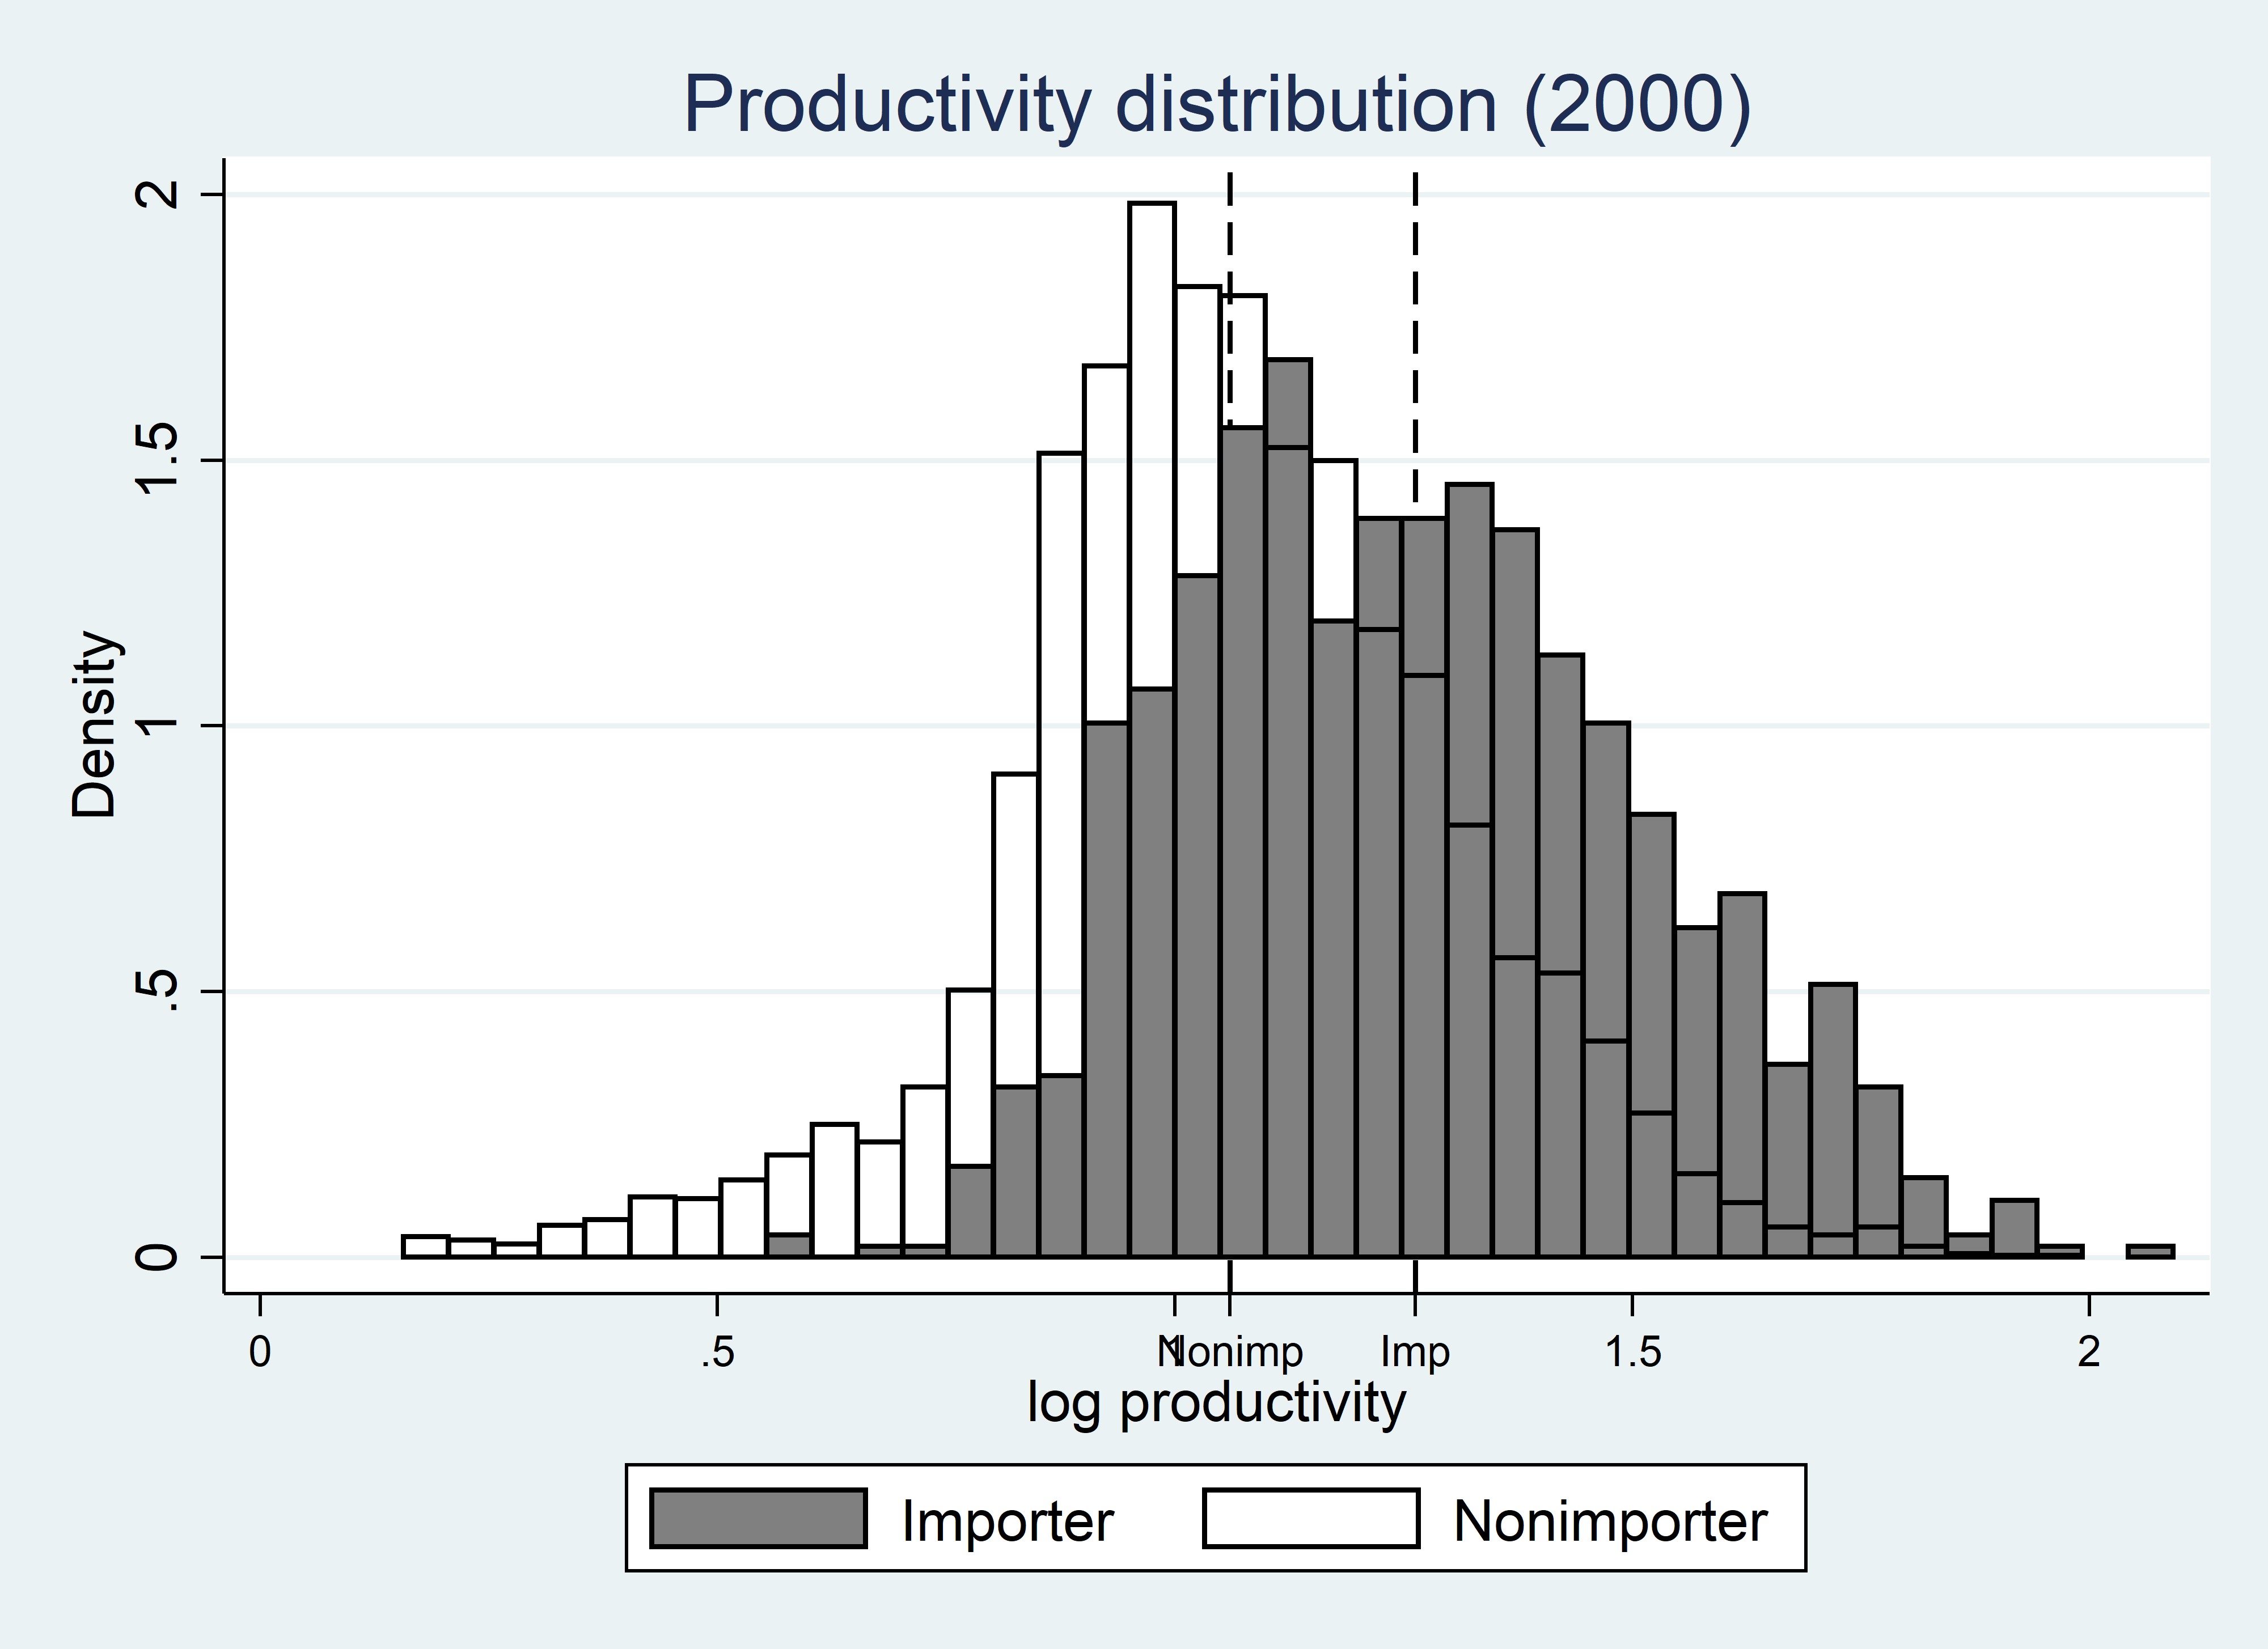
\includegraphics[width=0.6\textwidth]{prod_2000.png} 
\label{prod_2000}
\end{center}
\end{figure}

%\begin{figure}[h]
%\begin{center}
%\caption{Productivity distribution of importers and nonimporters (2000)}
%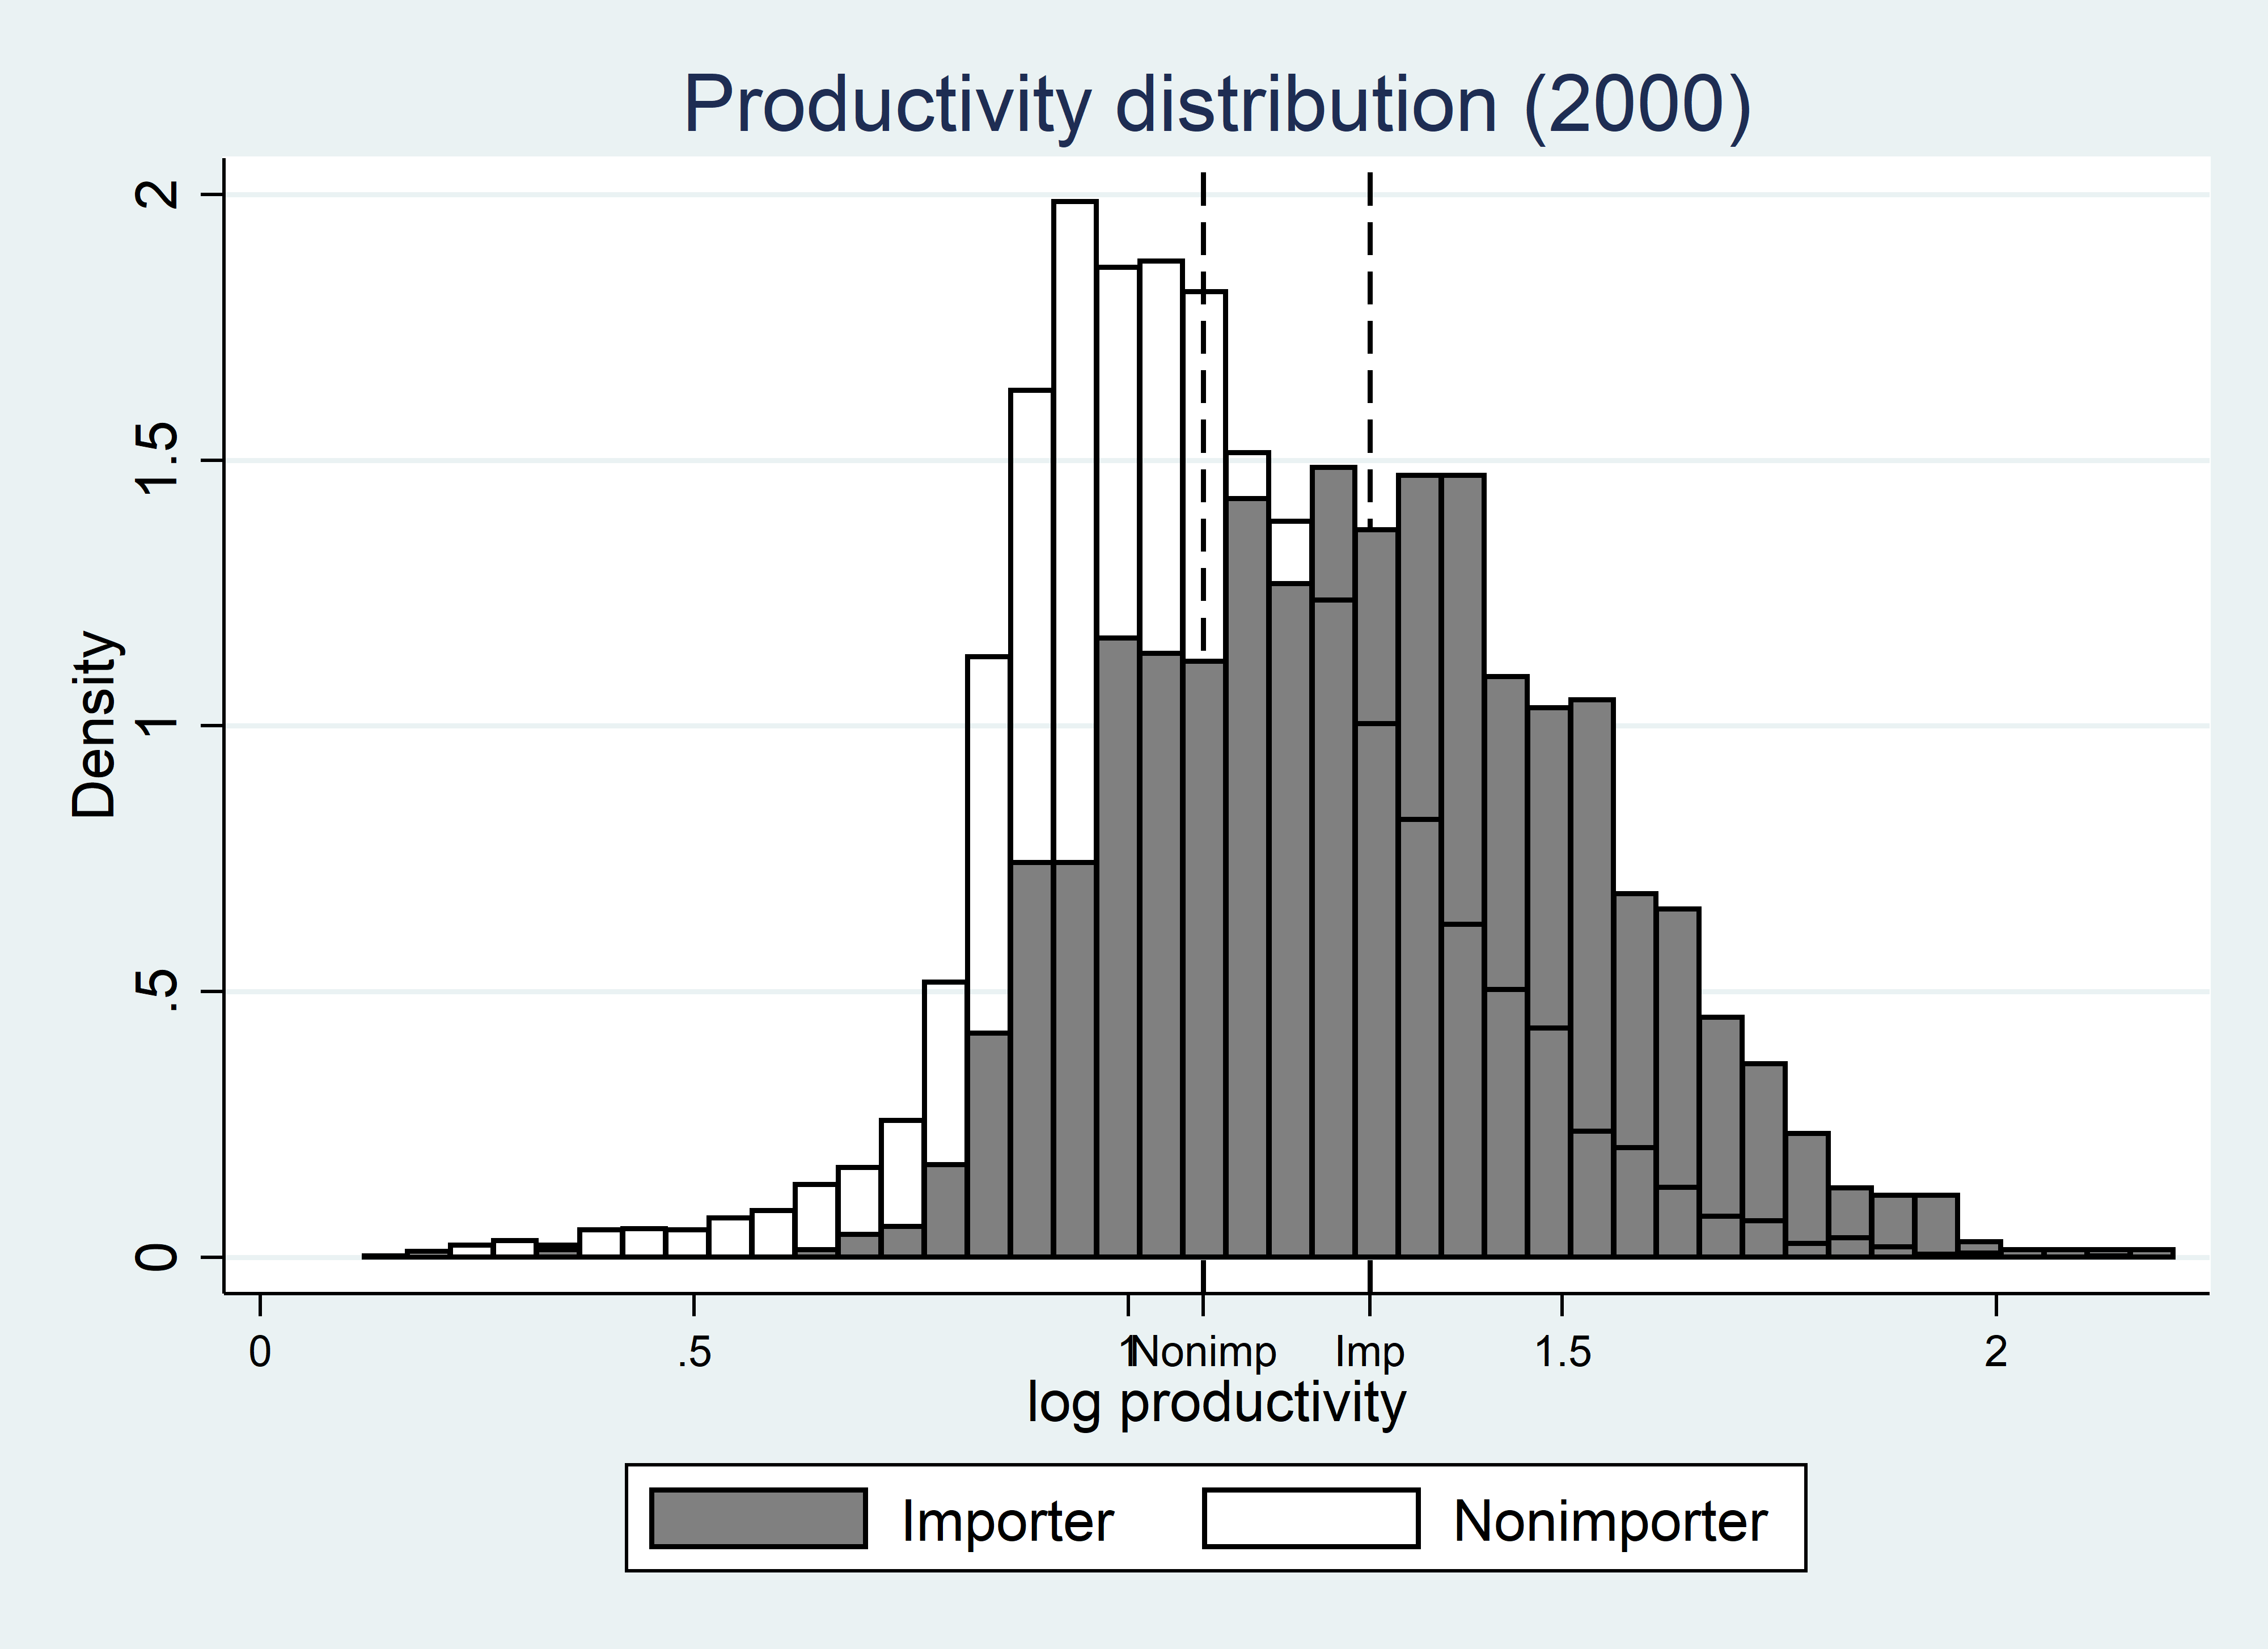
\includegraphics[width=0.6\textwidth]{prod_2003.png} 
%\end{center}
%\end{figure}

\begin{figure}[h]
\begin{center}
\caption{Productivity distribution of importers and nonimporters (2006)}
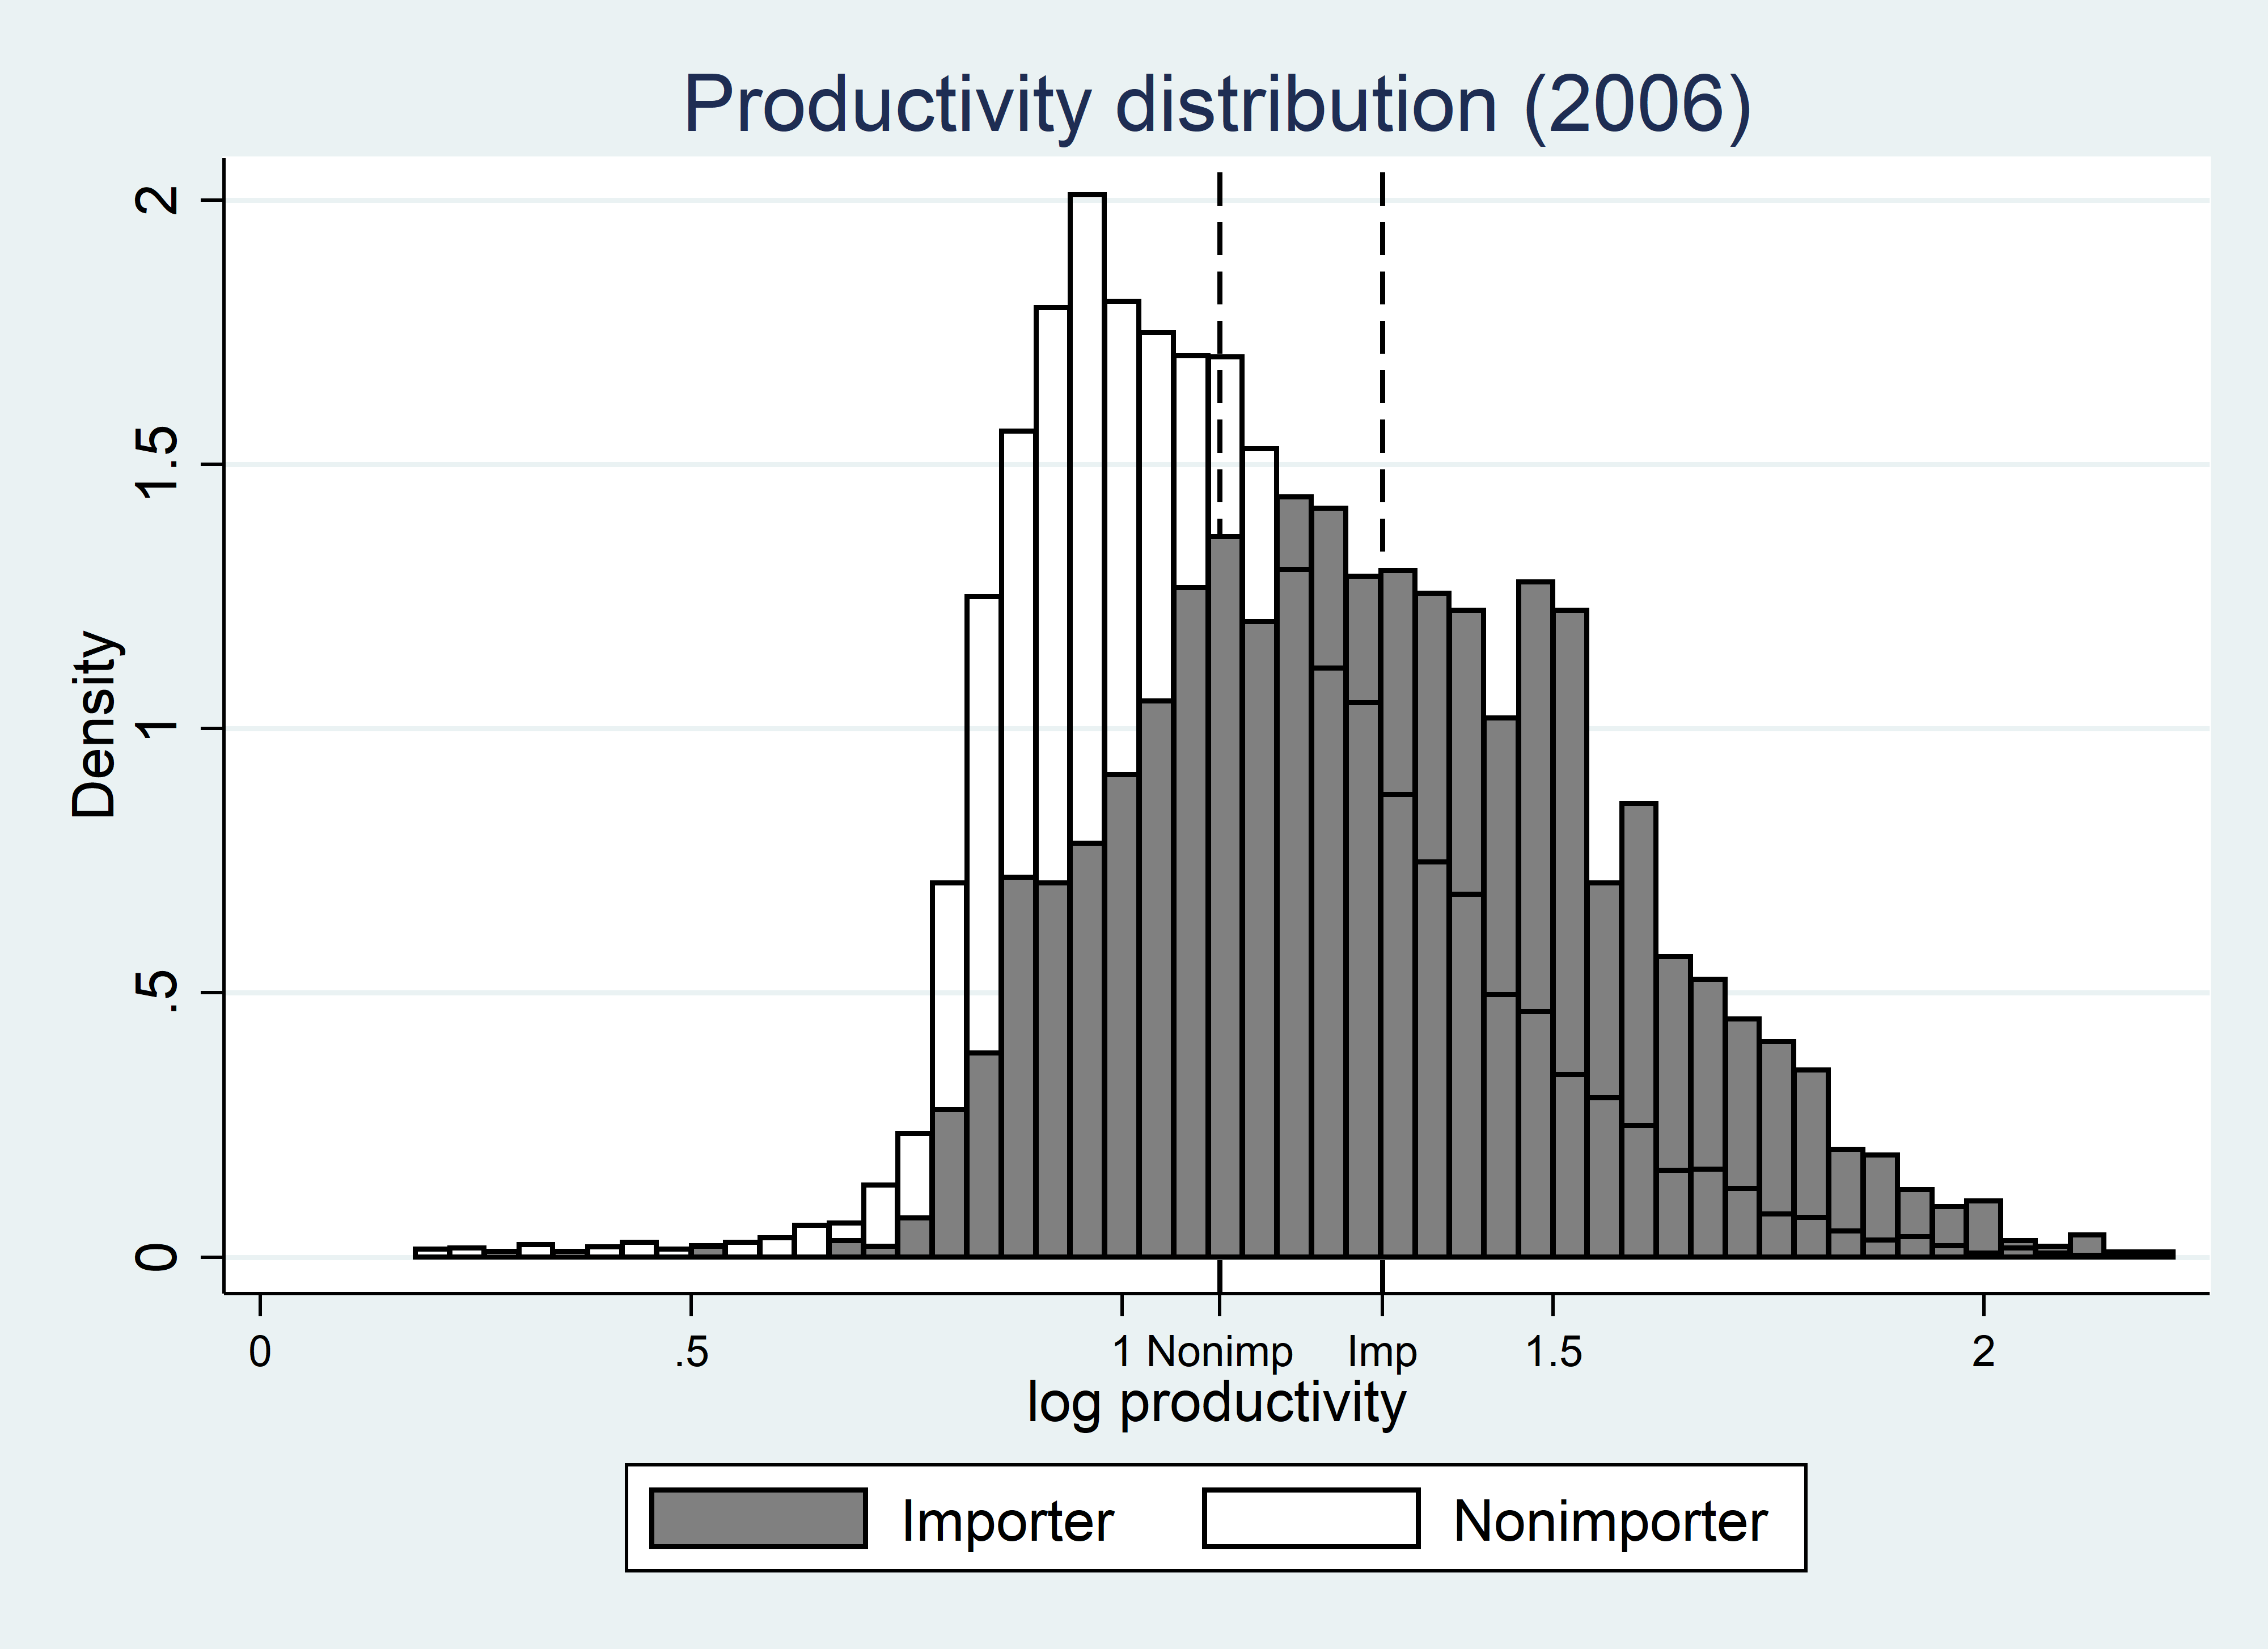
\includegraphics[width=0.6\textwidth]{prod_2006.png} 
\label{prod_2006}
\end{center}
\end{figure}

%%%%%%%%%%%%%%%%%%%%%%%%%%%%%%%%%%%%
\subsection{Second stage: Dynamic estimation}

TO BE CONTINUED


\end{appendices}




\end{document}  

 